\documentclass[25pt,a1paper]{tikzposter}
\geometry{paperwidth=80cm,paperheight=200cm}
%% Tikzposter is highly customizable: please see
%% https://bitbucket.org/surmann/tikzposter/downloads/styleguide.pdf

% a guide: https://roboticsconference.org/information/sample-poster2.pdf

%% Available themes: see also
%% https://bitbucket.org/surmann/tikzposter/downloads/themes.pdf
% \usetheme{Default}
% \usetheme{Rays}
 \usetheme{Basic}
% \usetheme{Simple}
%\usetheme{Envelope}
% \usetheme{Wave}
% \usetheme{Board}
% \usetheme{Autumn}
% \usetheme{Desert}

%% Further changes to the title etc is possible
% \usetitlestyle{Default}
% \usetitlestyle{Basic}
% \usetitlestyle{Empty}
% \usetitlestyle{Filled}
% \usetitlestyle{Envelope}
% \usetitlestyle{Wave}
% \usetitlestyle{verticalShading}

\usepackage{fontspec}
\setmainfont{FreeSerif}
\setsansfont{FreeSans}

\usepackage{anyfontsize}
 % Commands
 \newcommand{\bs}{\textbackslash}   % backslash
 \newcommand{\cmd}[1]{{\bf \color{red}#1}}   % highlights command


%    https://tex.stackexchange.com/questions/499066/how-to-increase-the-font-size-of-the-body-in-tikzposter

% https://taipeimedicaltourism.org/en/facility/detail/43
\author{Taipei Municipal Wanfang Hospital (Managed by Taipei Medical University}
\title{HEALTH CARE BEYOND
BORDERS}
\institute{Taiwan Medical Mission in the Republic of Somaliland}
%% Optional title graphic
\titlegraphic{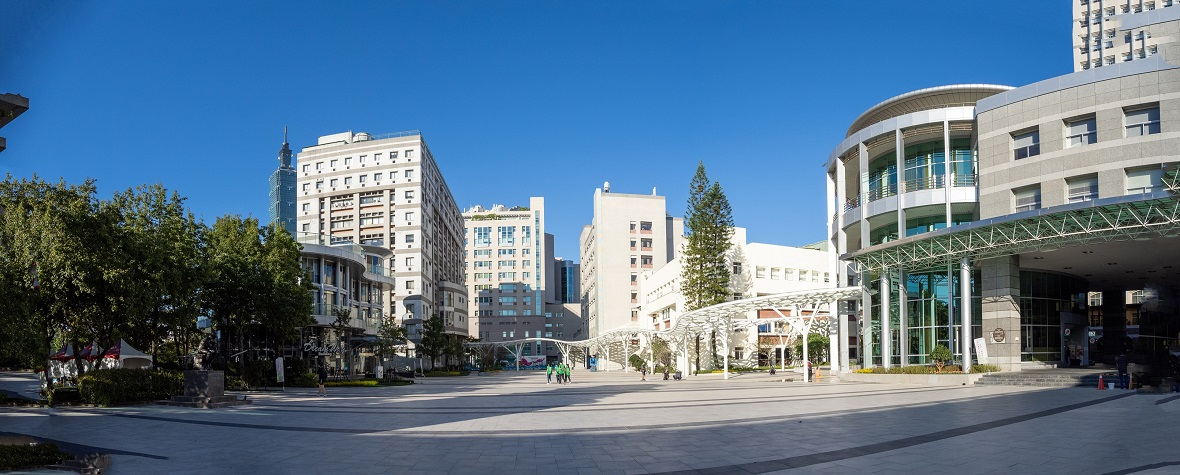
\includegraphics[width=0.55\linewidth]{TMU_square_4283326b11cfc41667f8cf91f5caaa21.jpg}}

% Taipei_5f994223a0add.jpg 
% https://www.mastersportal.com/search/master/medicine-health/taiwan
% 24cm
%% Uncomment to switch off tikzposter footer
% \tikzposterlatexaffectionproofoff

\begin{document}
\maketitle


\block{TMWH in TMU Healthcare System}{
\begin{itemize}

{\Large       %\fontsize{130}{50}

With outstanding medical research and accomplishments, Taipei Medical University (TMU) has established itself as one of Asia's leading institutions for medical education. The Taipei Medical University Hospital (TMUH), \underline{Wanfang Medical Center (TMWH)}, Shuang-Ho Hospital, TMU Taipei Cancer Center, Taipei Neuroscience Institute, and TMU LiHuiLi Hospital in Ningbo, China, are all part of the TMU Health System.
%TMU Healthcare System is better able to help medical professionals and patients in Taiwan and around the world by combining the existing clinical resources with cloud resources in their Information and Communications Technology (ICT) in medicine.\\

TMWH, as a private management of public hospital, has been operating by TMU since 1997 under the successful model of \underline{build, operation and transfer (BOT)}.

TMWH lays emphasis on high quality medical service comprehensively; moreover, it has obtained the certification of medical center and has received many awards since operated. Honorably, TMWH becomes the first hospital to get the accreditation of JCI for four times in 2015. That’s proved quality of service is our pride again.\\
% https://taipeimedicaltourism.org/en/facility/detail/43
More than 350 full-time doctors, more than 2000 other medical staff members, and 743 beds are available at TMWH. The majority of TMU-affiliated medical students and residents complete their internships at TMWH. 
In addition to its Health Examination Center, CyberKnife Center, Cancer Center, Obesity Prevention Center, Infertility Treatment Center, Laser Cosmetic Center, and Burn Center, TMWH is renowned for its specialties in neurosurgery, cardiology, orthopedics, hyperthermia therapy, and treatment of lower limbs lymphedema.\\
To help international visitors, TMWH has set up an international liaison center. Websites providing international medical services, travel preparation, hotel arrangements, direct admission, billing coordination, as well as help before to, during, and after hospitalization are among the services that are offered.


%From the beginning, our hospital visions were, to treat patients with respect, become a center of integrative medicine and provide comprehensive care for all and provide community-oriented service. 
As a renowned university hospital with a worldwide patients, TMWH is fully committed to offering the best service available.

} % end of \fontsize or \huge

%\item \#TMUtw 
%\item \#TaipeiMedicalUniversity 
%\item \#CloudICT
\item \#Telemedicine \#Bioinformatics
\item \#CardiovascularTreatment \textcolor{green}{\#JointReplacement}
\item \textcolor{green}{\#KidneyTransplant} % https://www.wanfang.gov.tw/p9_medical_detail.aspx?cu=592
\#CancerTreatment
\item \#daVinciSurgery \#AestheticMedicine
\item \textcolor{green}{\#MuslimMedical}
\item \#HealthExamination
%\item we try to do that.
\end{itemize}
}

\note[rotate=8, connection, width = 6cm, targetoffsetx=-15cm, targetoffsety=-16cm
% roundedcorners=15, 
]{Mashallah\\ ما شاء الله}

\begin{columns}

\column{0.7}
\block{What responsibilities does TMU have?}{
\begin{itemize}
TMU Spotlight showcases impressive outcomes from our partnership collaboration, research excellence, talent development, and the University’s commitment to making a positive social impact.\\
\underline{Humanity, integrity, innovation, teamwork, and service} are among TMU's core values.
% 核心價值
% 人文關懷(Humanity)        :以人為本,尊重生命,厚植人文與專業教育。
% 誠信正直(Integrity)          :誠實為上,正直當責,堅持互信的組織文化。
% 創新卓越(Innovation)      :勇於創新,承擔風險,追求卓越以引領時代。
% 團隊合作(Collaboration) :尊重多元,跨域協作,共創永續發展的目標。
% 社會服務(Service)            :熱忱服務,影響社會,促進人類健康與福祉。
 

%\item We try to do this. what?
%\item we try to do that.
\end{itemize}

\innerblock{TMU's Hospitals}{
% Figures of TMU
\begin{minipage}{0.45\linewidth}
  \centering %456
    \begin{tikzfigure}[]
    % TMWH
    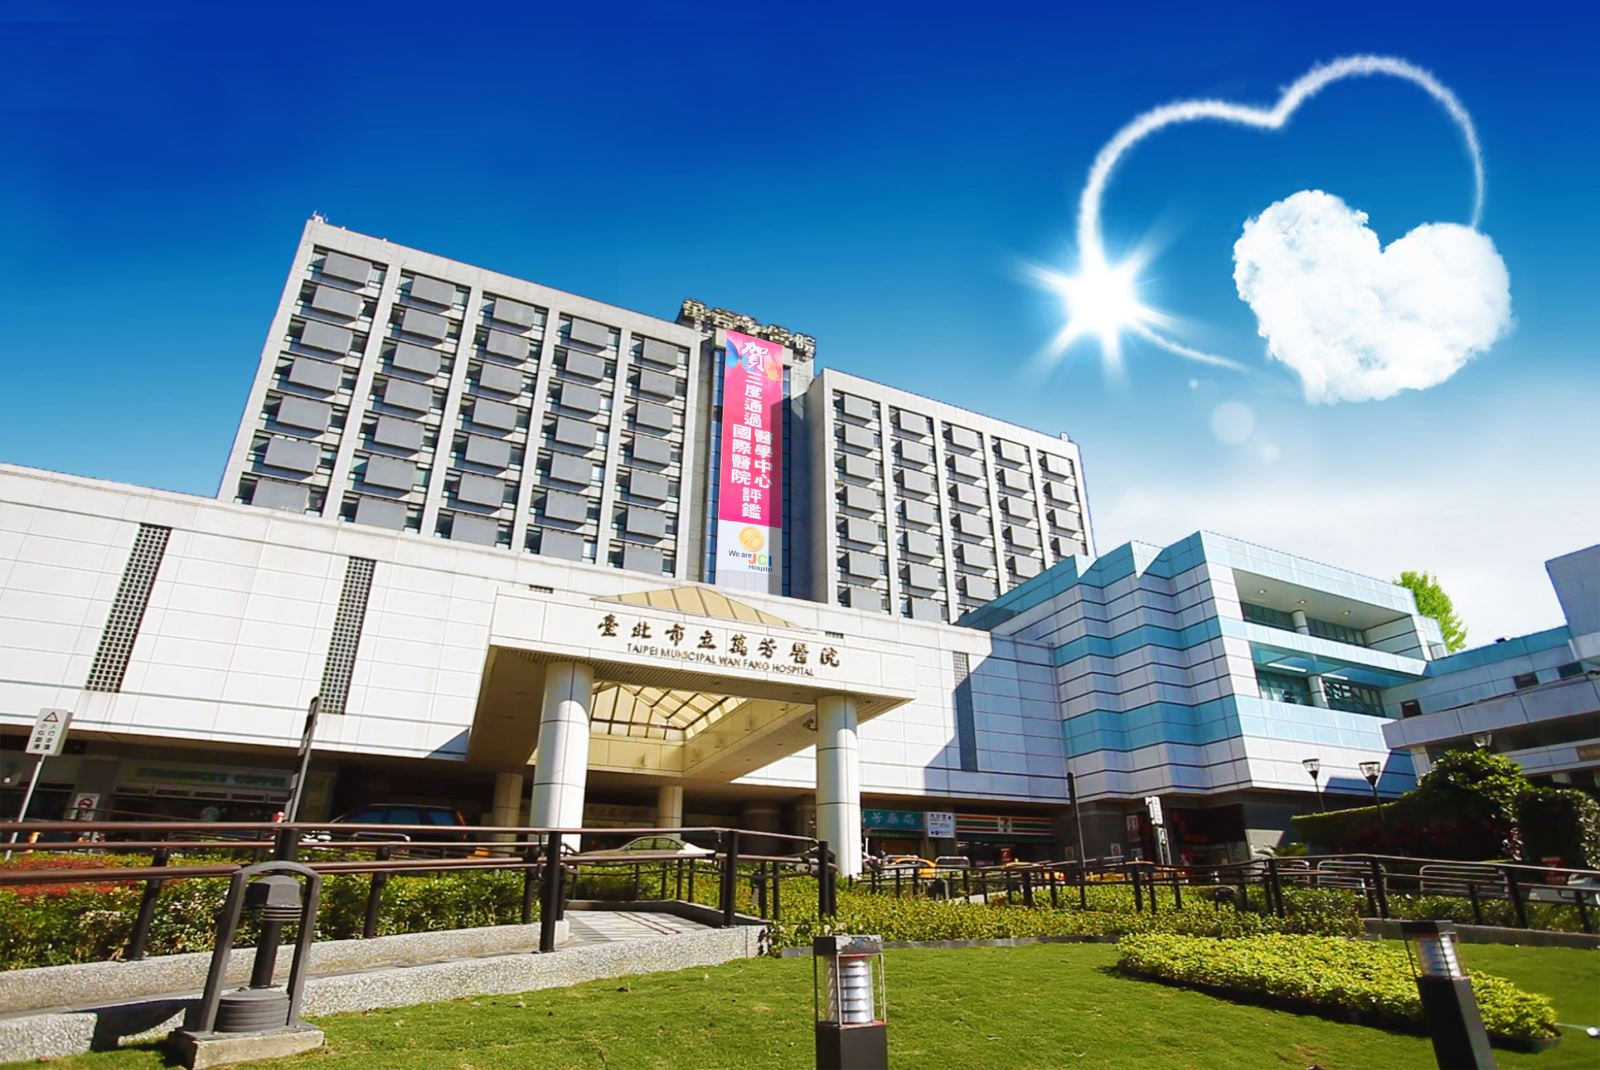
\includegraphics[width=0.8\linewidth]{5FAB9DAB-B258-4FC5-AED2-BB8F415E616F.jpeg}
    % TMUH
    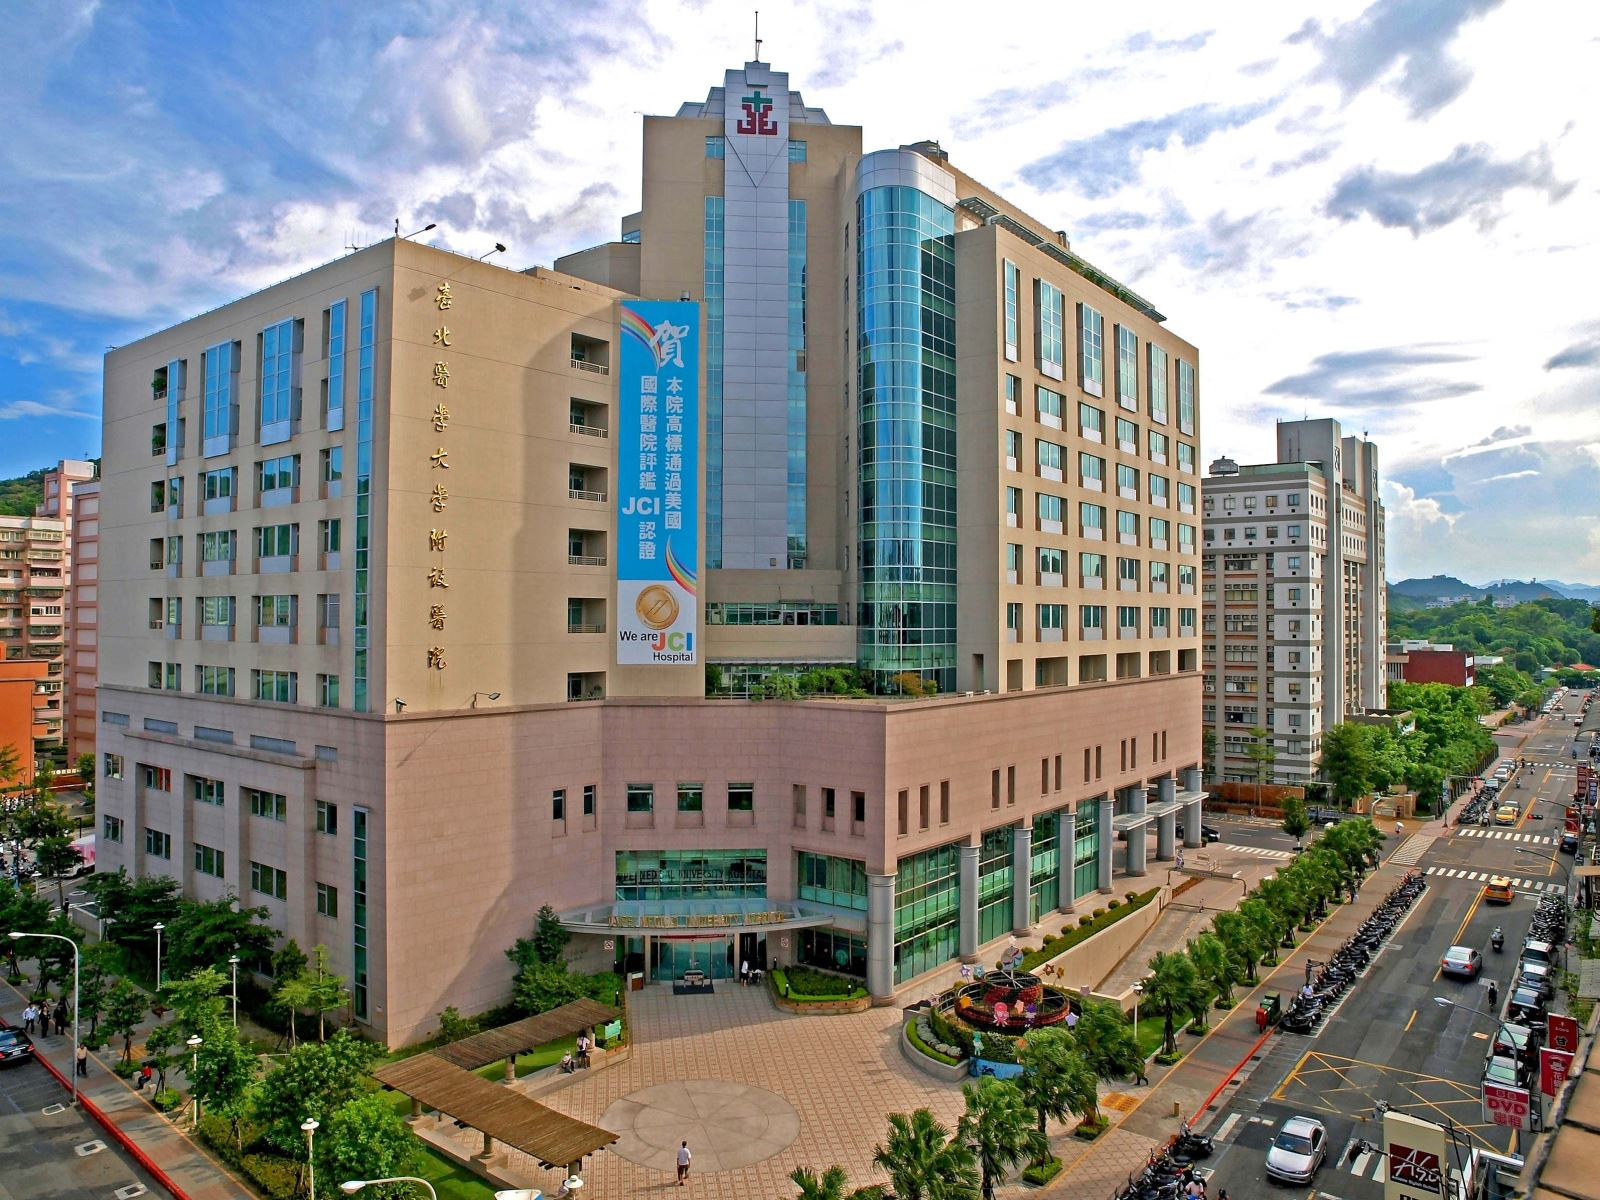
\includegraphics[width=0.8\linewidth]{5782F8B7-D58E-4601-A26D-18DFB462B6B8.jpeg}
    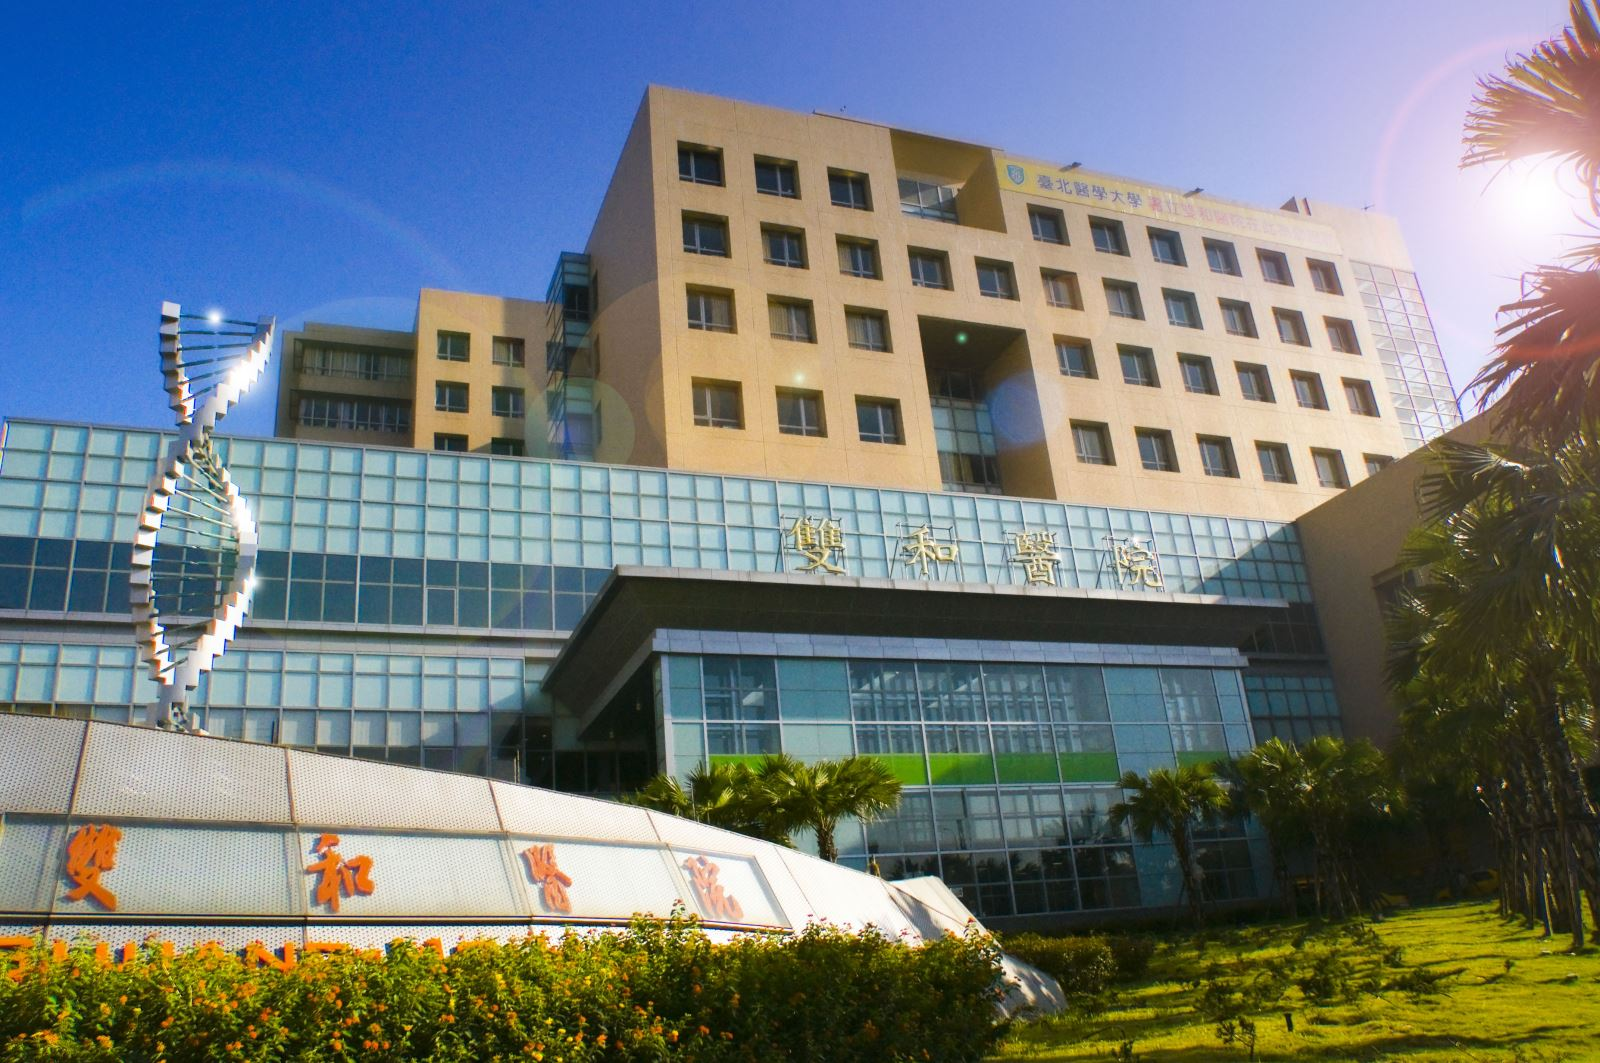
\includegraphics[width=0.8\linewidth]{10885B17-3876-4B24-B689-4B1ACDB21AB3.jpeg}
    \end{tikzfigure}
\end{minipage}\hfill
\begin{minipage}{0.45\linewidth}
  \centering
%\innerblock{TMU's Hospitals}{
    \begin{tikzfigure}[]
    %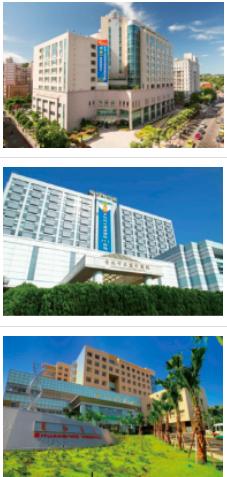
\includegraphics[width=0.5\linewidth]{TMU123.jpg}
    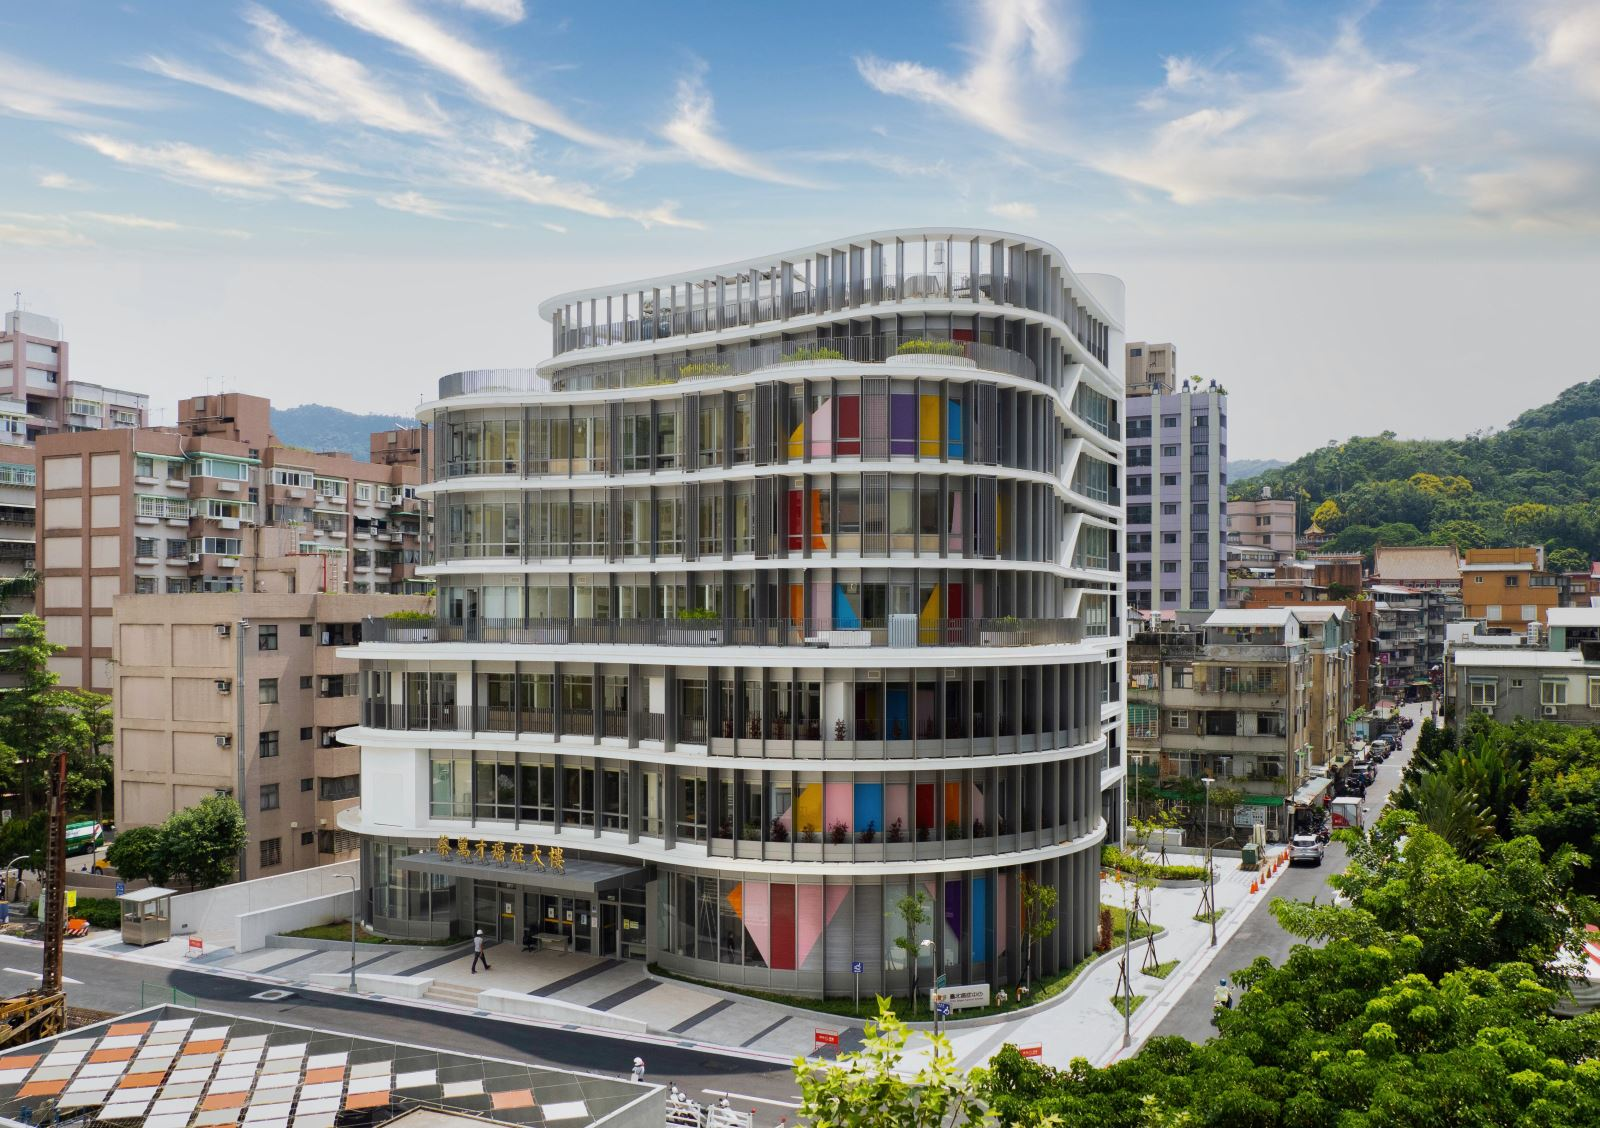
\includegraphics[width=0.85\linewidth]{295B6224-4030-47C6-9742-E3874C20445E.jpeg}
    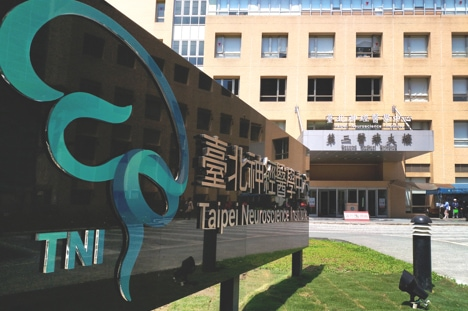
\includegraphics[width=0.85\linewidth]{6C597AEE-0ADA-4AC1-BA50-C500B9B911E0.jpeg}
    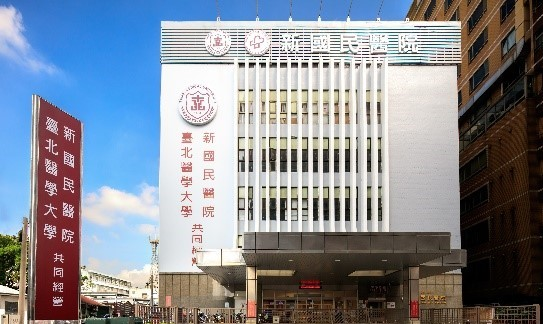
\includegraphics[width=0.85\linewidth]{17E0CB16-55CA-4F23-9A3A-F70CAE5FE133.jpeg}
\end{tikzfigure}
\end{minipage}
} % end of innerblock

} % end of block

\column{0.3}
\block{What TMWH does?}{
\begin{itemize}
\item To provide medical services based on special demand 
\item Clinical capacity building for health personnel individuals \item Public health research and improvements
\item Through \textbf{telemedicine} to provide international medical aid
\end{itemize}

% Taiwan Task Force For Medical Travel
\begin{tikzfigure}[Taiwan Task Force For Medical Travel]
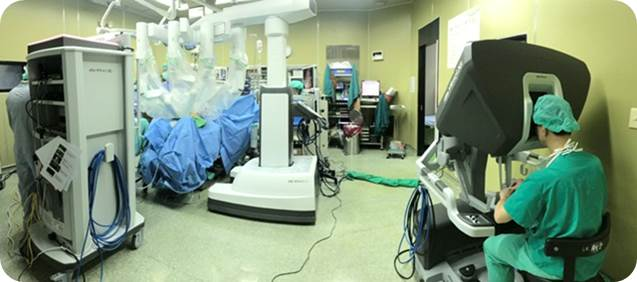
\includegraphics[width=\linewidth]{TMWH_daVinci.jpg}
\end{tikzfigure}

% thoracic surgery, otolaryngology, neurosurgery, general surgery, colorectal surgery, urology, obstetrics and gynecology, orthopedics
% http://www.taiwanhealthcare.com/product/40&path=60

Robotic arm assisted laparoscopic surgery (\textbf{da Vinci system}) is minimal invasive surgery for
urology, obstetrics & gynecology, general surgery (thyroid, breast), colorectal surgery.

{\tiny (* all photos courtesy of Public Relation \& Publishing Section, TMU Secretariat)}

}
\end{columns}

%%
\block{Breast Cancer Surgery in TMWH}{%
\begin{tikzfigure}[]
\includegraphics[width=0.7\linewidth]{0R5A3423.jpeg}
%{11001_TMWH_hybrideOT.jpg}
\end{tikzfigure}
}

%\block{TMU Main Campus}{%
%\begin{tikzfigure}[]
%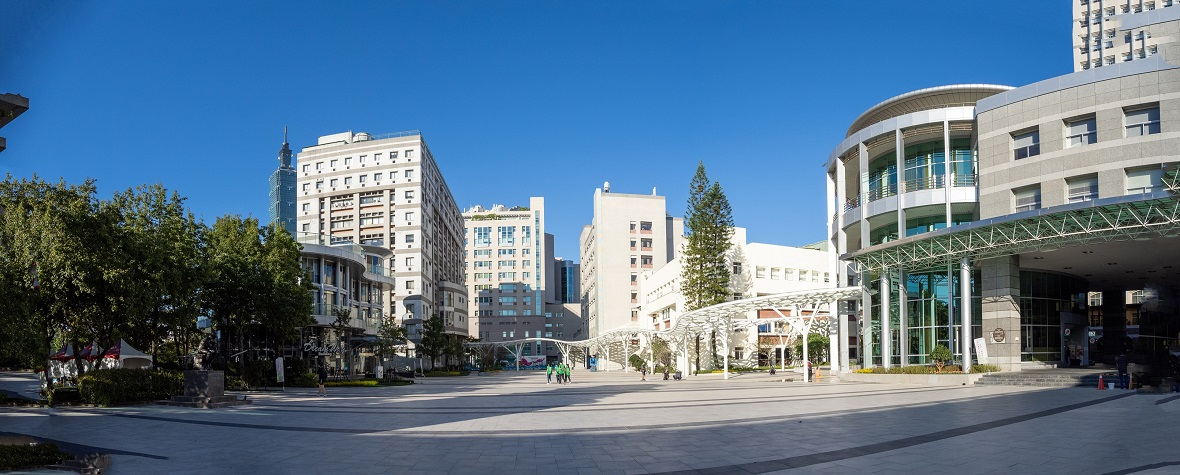
\includegraphics[width=\linewidth]{TMU_4283326b11cfc41667f8cf91f5caaa21.jpg}
%\end{tikzfigure}
%}


\block{TMWH Students and Doctors}{%

\begin{minipage}{0.23\linewidth}
  \centering
\begin{tikzfigure}[]
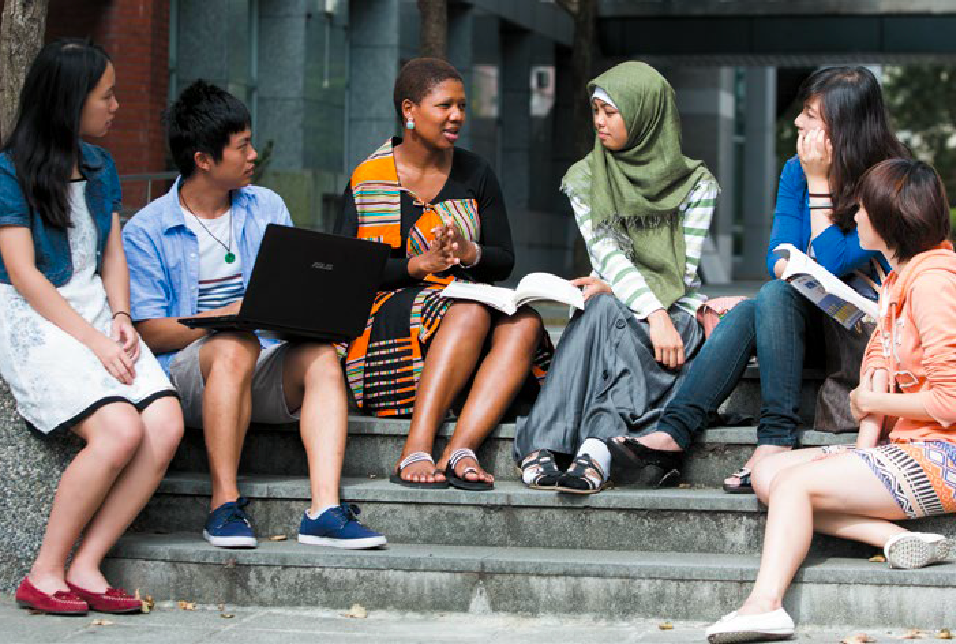
\includegraphics[width=\linewidth]{TMU_students.pdf}
\end{tikzfigure}

\end{minipage}\hfill
\begin{minipage}{0.23\linewidth}
  \centering
\begin{tikzfigure}[]
\includegraphics[width=\linewidth]{0R5A3306.jpeg}
\end{tikzfigure}
\end{minipage} \hfill
\begin{minipage}{0.23\linewidth}
  \centering
\begin{tikzfigure}[]
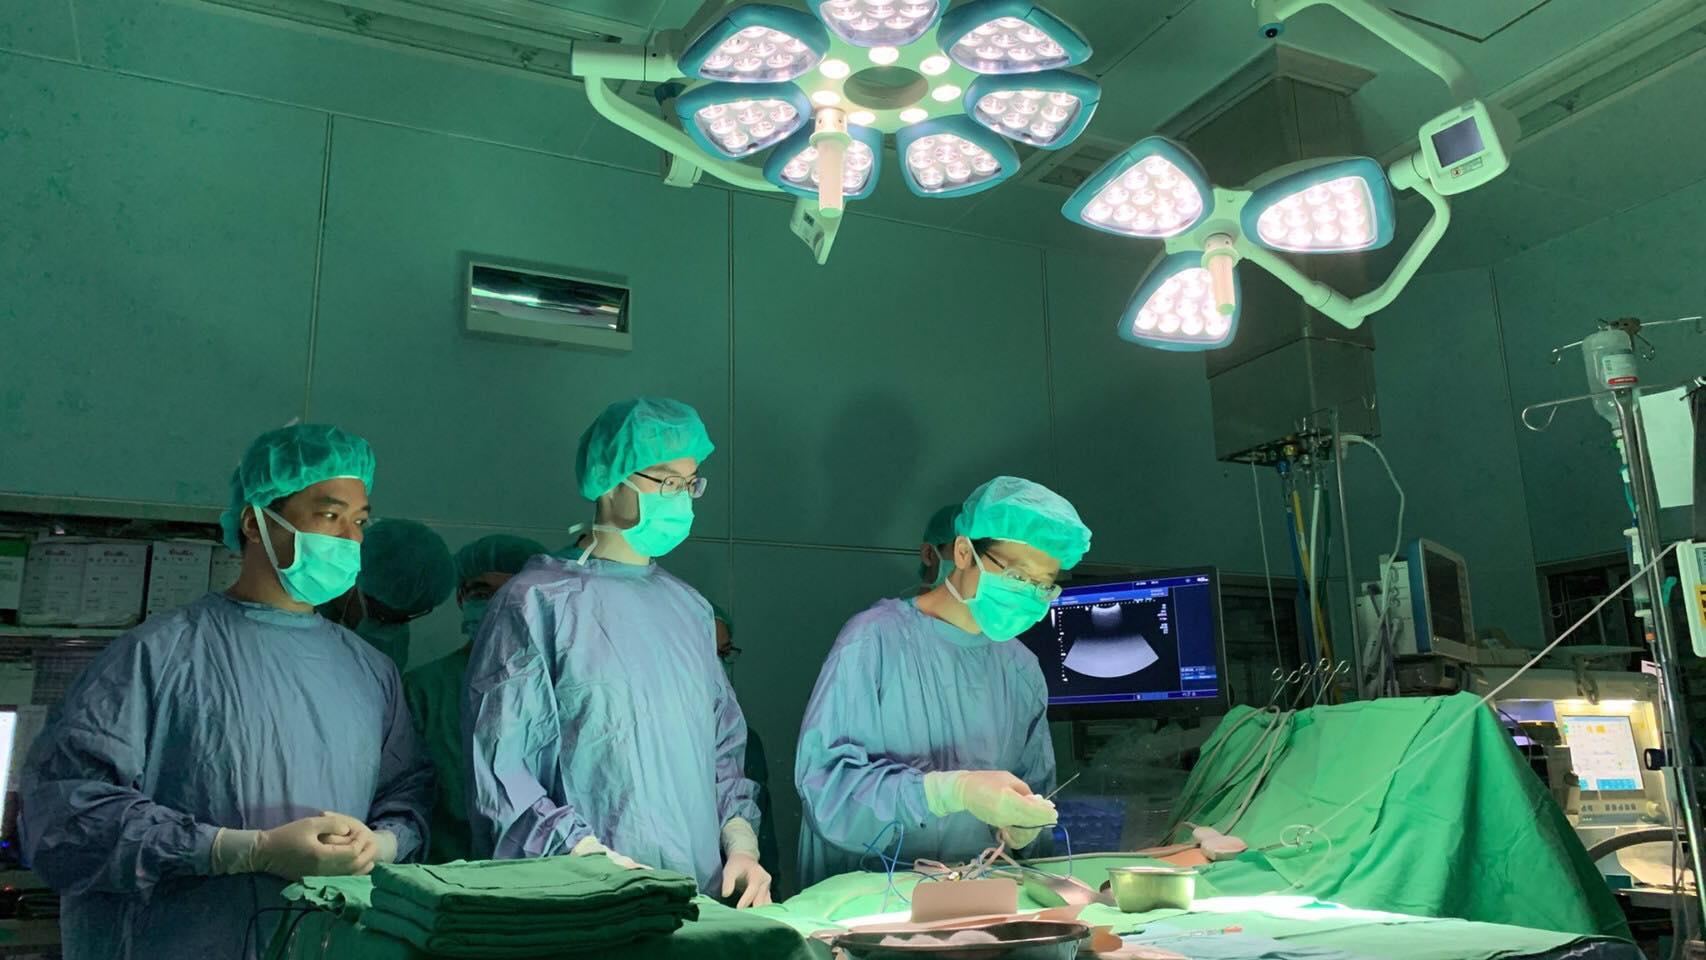
\includegraphics[width=\linewidth]{56541905_10219600203261606_5529101907710181376_o.jpeg}
\end{tikzfigure}

\end{minipage}\hfill
\begin{minipage}{0.23\linewidth}
  \centering
\begin{tikzfigure}[]
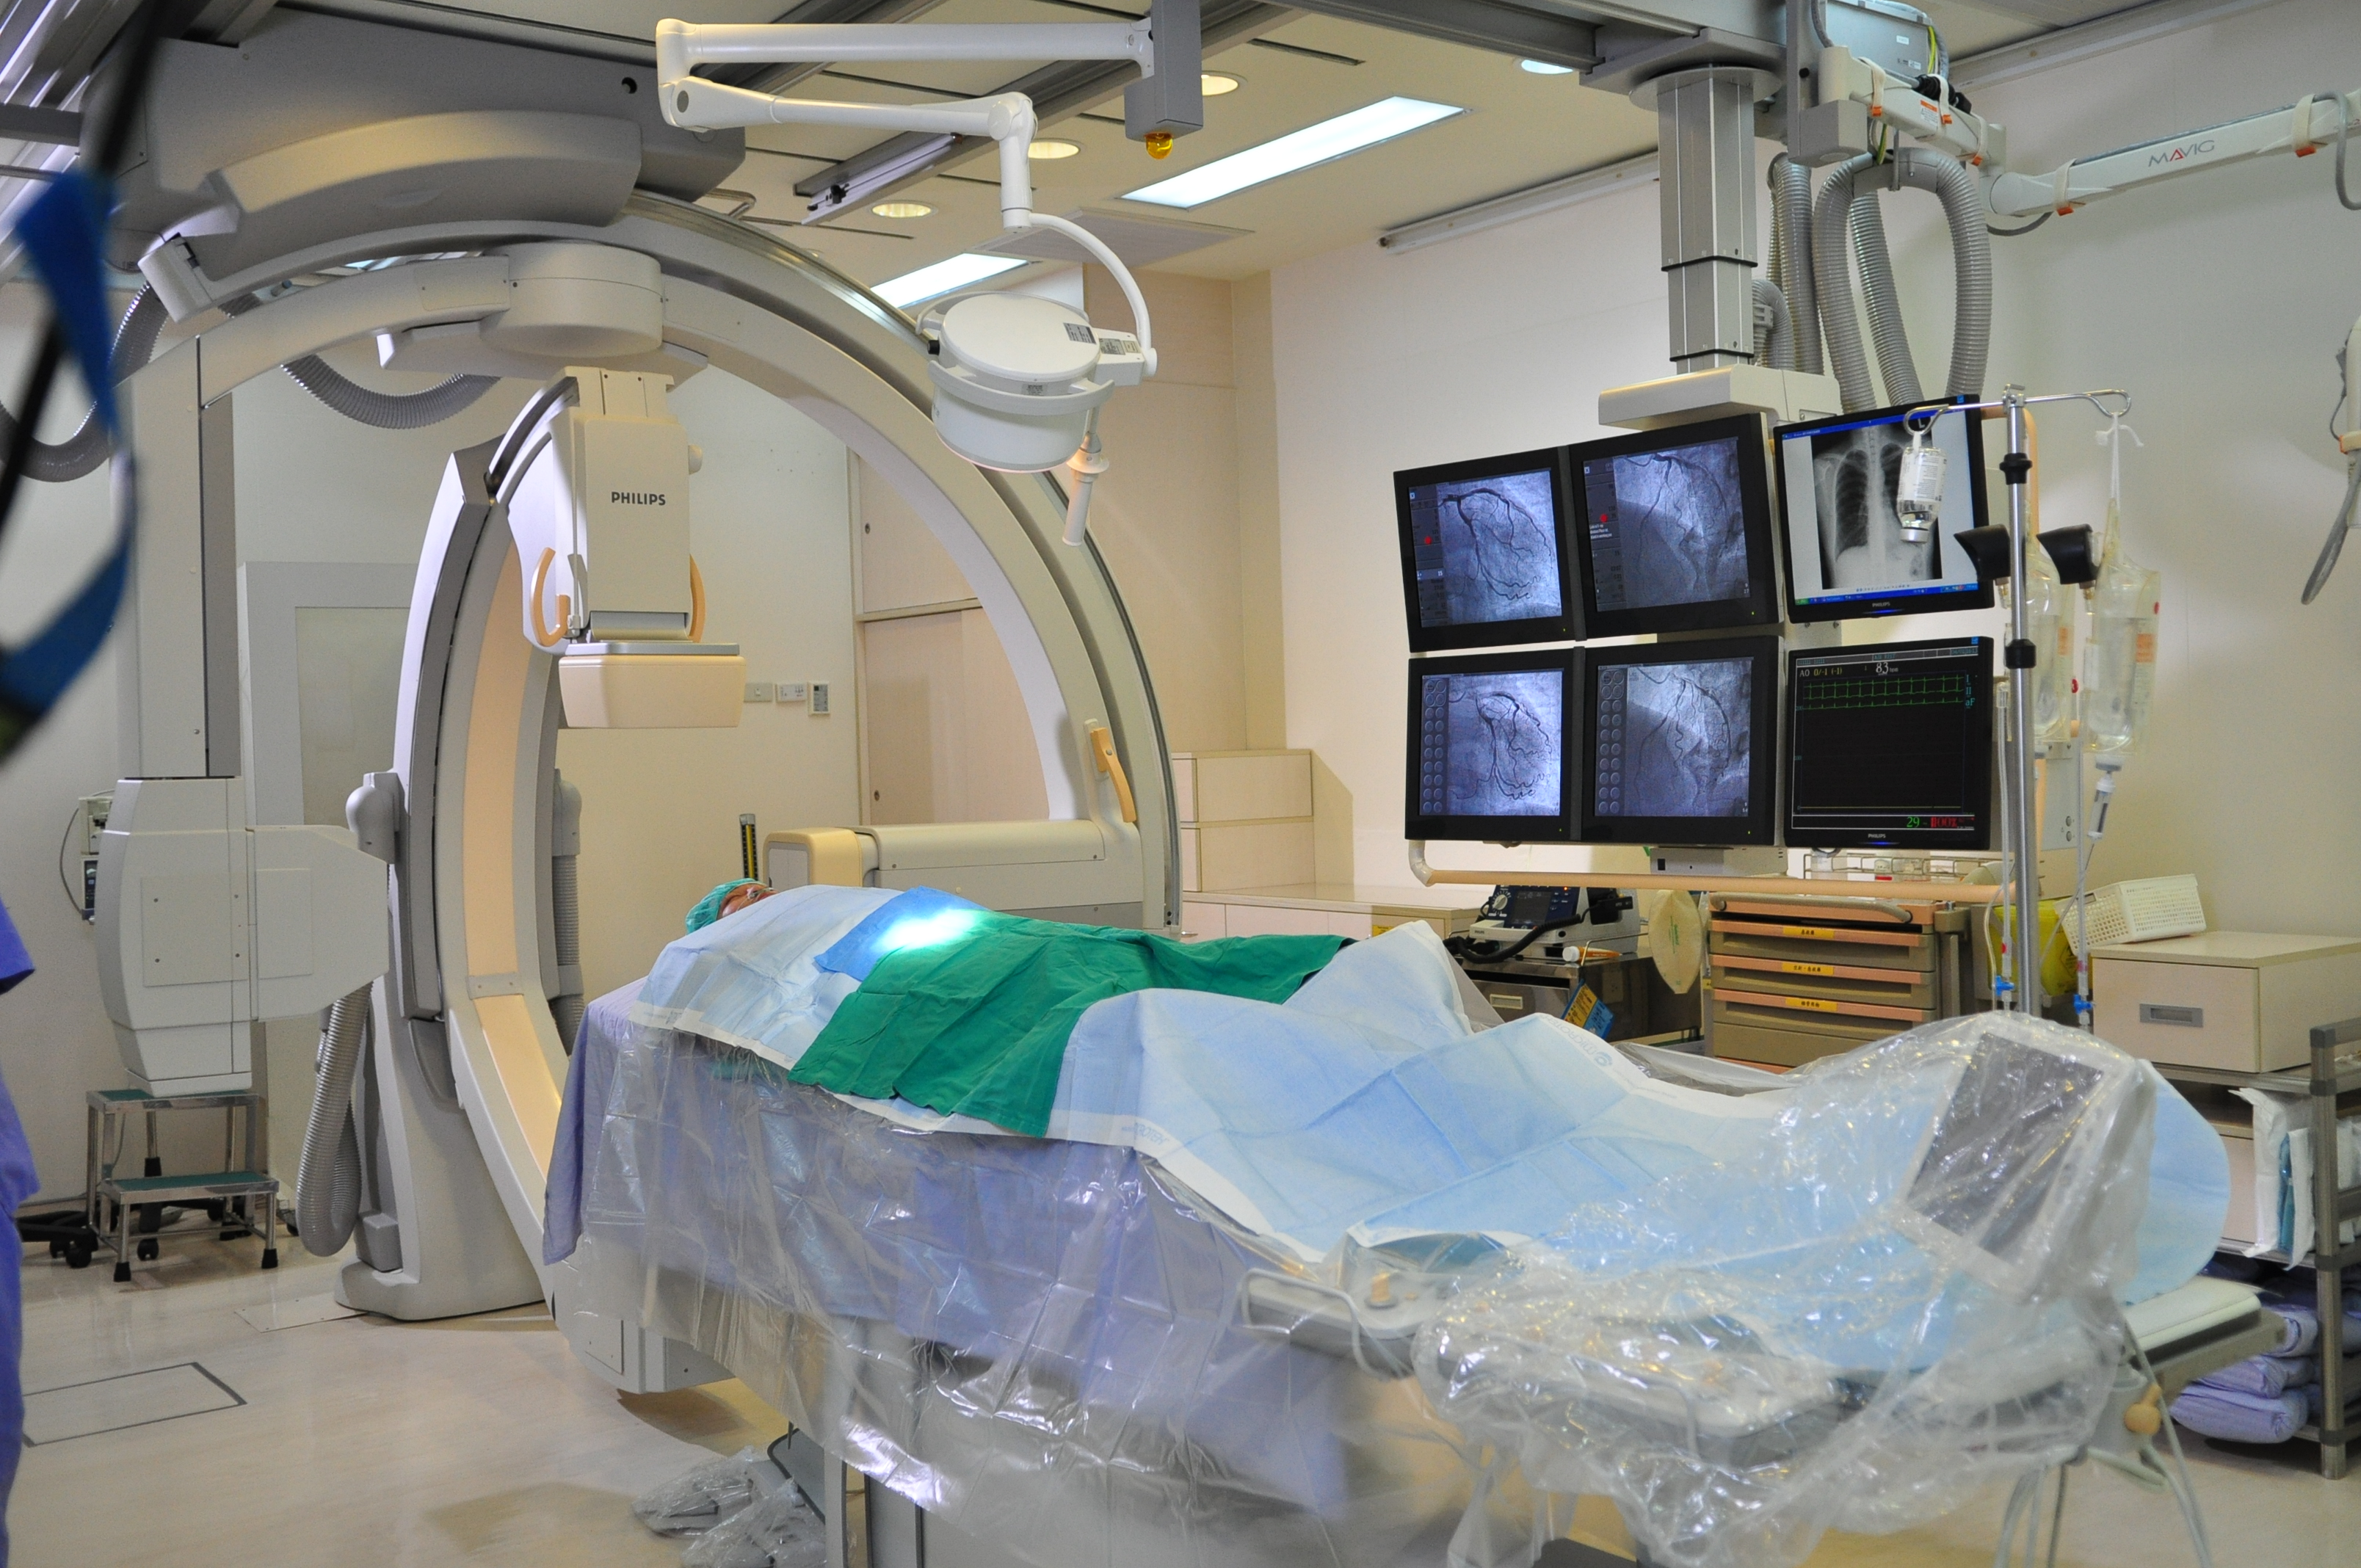
\includegraphics[width=\linewidth]{DSC_0385.jpeg}
\end{tikzfigure}
\end{minipage}


} % end of block


\block{Welcome to Taipei}{%
\begin{minipage}{0.3\linewidth}
  \centering
    \begin{tikzfigure}[International Scholar]
    
\includegraphics[width=0.5\linewidth]{TMU_QR_sholar.png}
%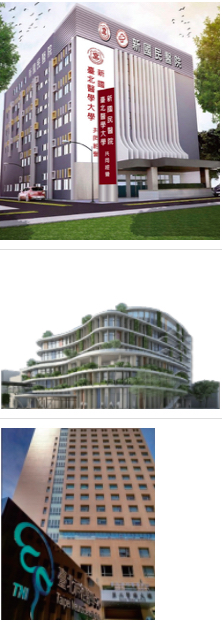
\includegraphics[width=0.5\linewidth]{TMU456.jpg}
    \end{tikzfigure}
\end{minipage}\hfill
\begin{minipage}{0.3\linewidth}
  \centering
\begin{tikzfigure}[]
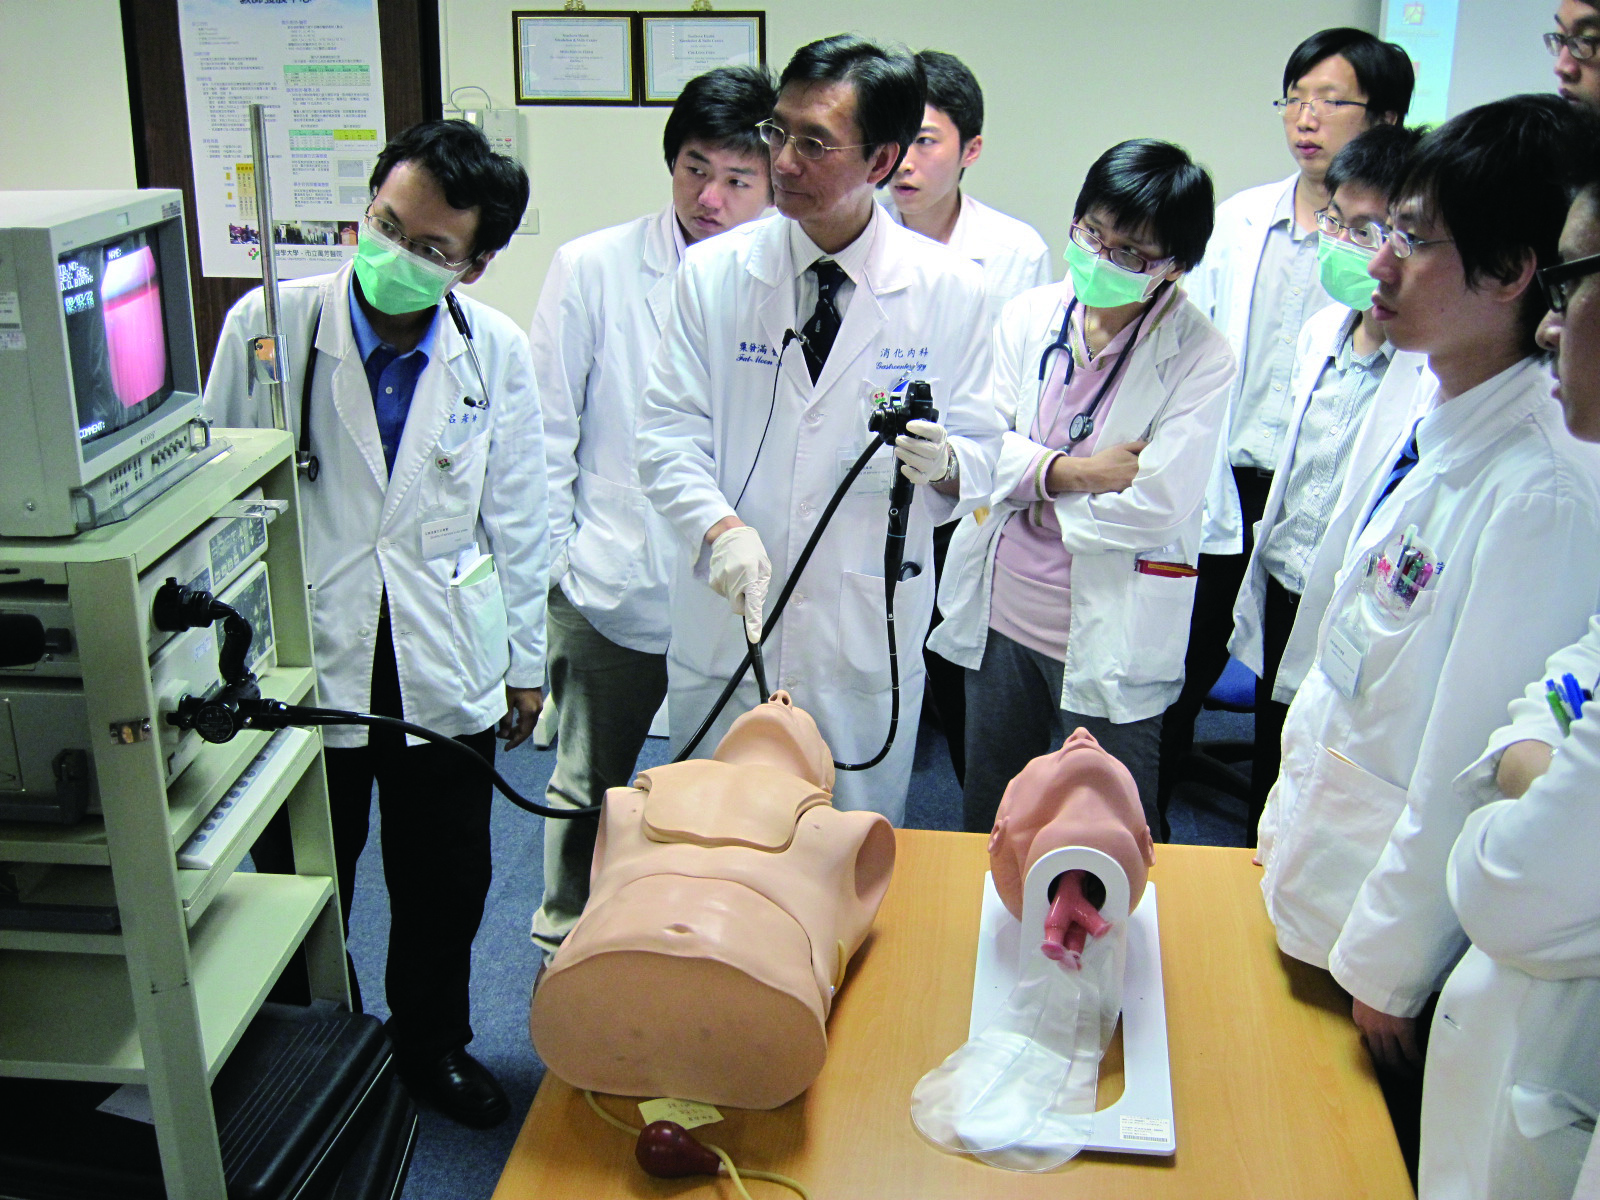
\includegraphics[width=\linewidth]{2萬芳醫院中英文簡介照片.jpg}
\end{tikzfigure}  
\end{minipage}\hfill
\begin{minipage}{0.3\linewidth}
  \centering
\begin{tikzfigure}[Medical Tourism]

\includegraphics[width=0.4\linewidth]{qrcode.66164813.jpg}
\end{tikzfigure}
\end{minipage}

%(* photos courtesy of Studyportals B.V., and Public Relation \& Publishing Section, TMU Secretariat)
} % end of block
\end{document}